% ----------------------------------------------------------
% Introdução 
% Capítulo sem numeração, mas presente no Sumário
% ----------------------------------------------------------

\chapter*[Introdução]{Introdução}
\addcontentsline{toc}{chapter}{Introdução}

Um computador moderno consiste em um emaranhado de peças que contém um ou mais processadores, alguma memória principal, alguma memória secundaria, interfaces de rede diversos periféricos como impressoras, teclado, mouse, monitor e vários outros dispositivos de entrada e saída. Podemos dizer que este é um sistema complexo, para realizar a desafiadora maratona que é compreender como cada parte funciona e gerenciar com maestria esses componentes é um grande desafio \cite{Tanenbaum2016}.\\
Para isso os computadores modernos são equipados com um SO esse dispositivo de \emph{software} tem a função de fornecer uma plataforma simples e limpa para o usuário de forma a ajuda-lo nas entradas e saídas de dados. Em uma visão simplista podemos ver na figura \ref{fig:figura1} onde o SO se encontra em relação entre \emph{hardware} e o usuário \cite{Tanenbaum2016}. 

\begin{figure}[htpb]
    \centering
   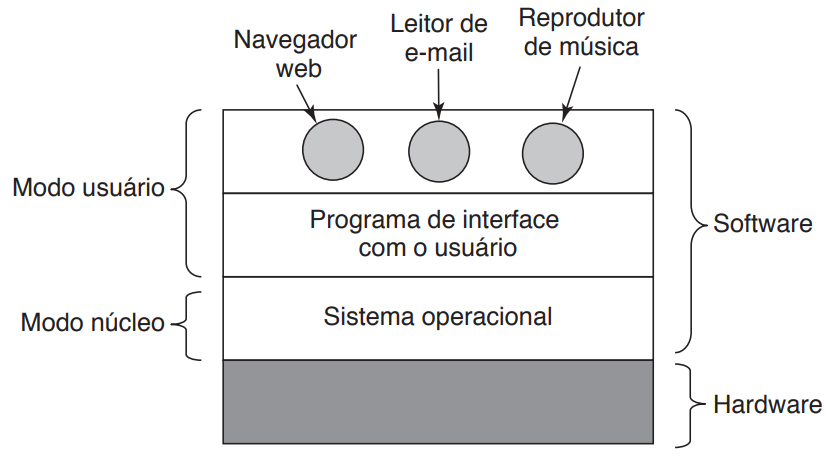
\includegraphics[scale=.4]{imagens/figura1.png}
   \caption{Onde o sistema operacional se encaixa. \cite{Tanenbaum2016}}
   \label{fig:figura1}
\end{figure}

Inicialmente a ideia que temos de um SO é a visão que temos dos ditos sistemas operativos que temos conhecimento que podem ser \emph{Windows}, \emph{Linux}, \emph{FreeBSD}, ou \emph{OS X} mas normalmente a forma de interagir com diretamente com o sistema é através de terminais comumente conhecidos como shell (interpretadores de comando) isto quando baseado em texto ou \emph{GUI (Graphical User Interface)} quando em modo gráfico \cite{Tanenbaum2016}.\\
Um sistema operacional é projetado para ocultar as particularidades de \emph{hardware} (ditas "de baixo nível") e assim criar uma máquina abstrata que fornece às aplicações serviços compreensíveis ao usuário (ditas "de alto nível") \cite{Comer2012}.\\
Assim o sistema trabalha em dois estados o modo núcleo e o modo usuário. Sendo que no modo núcleo (também chamado modo supervisor ou \emph{Kernel mode}). O sistema tem acesso completo aos recursos seja de ao \emph{hardware} ou \emph{software} e pode executar qualquer instrução que a máquina for capaz de executar \cite{Tanenbaum2016}, \cite{linfo2007}.\\
Quando o sistema está em modo \emph{kernel} é considerado que as execuções são de uma fonte confiável e, portanto, pode executar quaisquer instruções e fazer referência a quaisquer endereços de memória (ou seja, locais na memória). O \emph{kernel} tem total controle sobre o sistema e trata todos os outros \emph{software}s como programas não confiáveis, assim todas as operações em modo usuário que necessitem alterar o sistema solicitam ao uso do \emph{kernel} por meio de uma chamada de sistema  para executar instruções privilegiadas, como criação de processos ou operações de entrada / saída \cite{Tanenbaum2016}, \cite{linfo2007}.\\

Neste trabalho iremos trabalhar com o sistemas baseados em \emph{Linux} para servidores mas é importante entender um pouco da evolução desse sistema.

Em meados da década de 60 uma iniciativa conjunta do \emph{MIT}, da \emph{Bell Labs}  e da \emph{General Electric} decidiram embarcar no desenvolvimento de um “computador utilitário”, isto é, uma máquina que daria suporte a algumas centenas de usuários simultâneos em pouco tempo nasce o projeto MULTICS (Serviço de Computação e Informação Multiplexada) \cite{Tanenbaum2016}.\\
O MULTICS foi projetado para ser um sucesso com suporte para centenas de usuários em uma máquina apenas um pouco mais poderosa do que um PC baseado no 386 da \emph{Intel}. Mas transformá lo em um produto final de fácil comercialização não foi amarga realidade \cite{Tanenbaum2016}.\\
A \emph{Bell Labs} abandonou o projeto, e a \emph{General Electric} abandonou completamente o negócio dos computadores. Entretanto, o \emph{MIT} persistiu e finalmente colocou o MULTICS para funcionar.E foi instalado por mais ou menos 80 empresas e universidades importantes mundo afora \cite{Tanenbaum2016}.\\
Um dos cientistas da \emph{Bell Labs} que havia trabalhado no projeto MULTICS, Ken Thompson, decidiu escrever uma versão despojada e para um usuário do MULTICS. Esse trabalho mais tarde desenvolveu-se no sistema operacional UNIX, que se tornou popular no mundo acadêmico, em agências do governo e em muitas empresas \cite{Tanenbaum2016}.\\
Em 1987, Andrew Tanenbaum lançou um pequeno clone do UNIX, chamado MINIX, para fins educacionais. Em termos funcionais, o MINIX é muito similar ao UNIX \cite{Tanenbaum2016}.\\
Em 1991 Linus Torvalds começou um projeto inicialmente um emulador de terminal que era utilizado para acessar os servidores em UNIX da universidade Helsinki. Ele escreveu o código para especificamente  para o \emph{hardware} que utilizava um computador com um processador 80386 ele realizou o desenvolvimento no minix usando o \emph{GNU C compiler} \cite{Torvalds1991}, \cite{Torvalds1993}, \cite{torvalds2002}.\\
O \emph{Linux} também é distribuído sob uma licença de código aberto. O código aberto segue estes locatários principais:
\begin{itemize}
    \item A liberdade de executar o programa, para qualquer propósito.
    \item A liberdade de estudar como o programa funciona e alterá-lo para que ele faça o que você deseja.
    \item A liberdade de redistribuir cópias para que você possa ajudar seu vizinho.
    \item A liberdade de distribuir cópias de suas versões modificadas para terceiros.
\end{itemize}
Esses pontos são cruciais para entender a ideia por trás do \emph{Linux}. O \emph{Linux} se transformou em um sistema de fácil acesso. Com a grande liberdade de se poder modificar o sistema ele proporcionou a criação de diversas distribuições uma vez que qualquer usuário pode criar uma que atenda a suas necessidades \cite{LinuxFundationWIL}.\\
Nos próximos sessões  iremos discutir sobre o sistema e aprofundar no \emph{Linux} para assim entender, suas funcionalidade, modo de funcionamento e  quais suas principais atuações.\\









%\section*{Figuras}\label{sec:figuras}
%\addcontentsline{toc}{section}{figuras}

% \section*{Tabelas}\label{sec:tabelas}
% \addcontentsline{toc}{section}{tabelas}

%\section*{Motivação}\label{sec:motivacao}
%\addcontentsline{toc}{section}{Motivação}

%\section*{Objetivos}\label{sec:objetivos}
%\addcontentsline{toc}{section}{Objetivos}


